!en \section{Let there be light!}
!de \section{Es werde Licht!}

!en The first sample in this chapter is the smallest program I can think of which does something.

!de Das erste Beispiel in diesem Kapitel ist das kleinste Programm, das ich mir vorstellen kann, das tatsächlich auch etwas sichtbares tut.



!en This program will switch on the LED on your Arduino pin 13.

!de Es schaltet die LED am Arduinoanschluss 13 ein.



!en Programming in Assembler means you're in control. But as you know, power requires knowledge and responsibility. If you're entering the world of assembly programming, you have absolute power if you wish to or not. Consequently you need knowledge to become responsible.

!de In Assembler Programmieren heisst, Du hast die Macht! Aber wie wir wissen, erfordert Macht Wissen und Verantwortungsbewusstsein. Jemand der Micro Controller in Assembler programmiert, hat die absolute Macht, ob er es will oder nicht! Demzufolge ist ein Mindestmass an Fachwissen erforderlich um verantwortlich zu handeln.



!en At first you need to know what 'Arduino pin 13' really means. As consequence of the Arduino design it is not pin 13 on your \at. Knowing this is yet the half way thru. Knowing the pin is a step you need to know if are working with a plain chip. What you need to know is the micro controllers internal addressing for Arduino pin 13. To find out, look at \url{http://www.arduino.cc/hu/Hacking/PinMapping}.

!de Als erstes musste Du wissen, was Anschluss 13 am Arduino in Wirklichkeit heisst. Infolge des Arduinodesigns ist Anschluss 13 am Arduino nicht Pin 13 am \at. Das zu wissen ist erst die halbe Miete. Das tatsächliche Pin am \at zu kennen ist erforderlich um mit dem blanken Chip zu arbeiten. Was Du ausserdem wissen musst ist, wie dieser Anschluss im Micro Controller adressiert werden muss. Um das alles heraus zu finden gibt es ein sehr schönes Schaubild: \url{http://www.arduino.cc/hu/Hacking/PinMapping}


\begin{figure}[htbp]
  \centering
  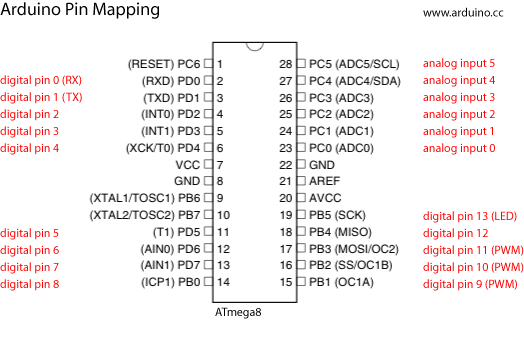
\includegraphics[width=120mm]{Media/www-arduino-cc_Arduino-To-Atmega8-Pins.png}
  \caption{Arduino to \at pins}
  \label{arduino-to-atmega-pins}
\end{figure}

!en After we know everything we need to know to be responsible, we generate our 8byte program that will set our 'LED 13' under power.

!de Nachdem wir zunächst vermutlich genug wissen um verantwortungsvoll zu handeln, programmieren wir unser 8 Byte grosses Programm , dass 'Adruino LED 13' erleuchtet.


\begin{lstlisting}
; LED/S000_let-there-be-light.asm

.DEVICE atmega8

.org 0x0000
            rjmp    start 

start:
            sbi     DDRB,         5
            sbi     PORTB,        5
            
main:
            rjmp    main
\end{lstlisting}

!en As simple as the program is, I believe there is some need for explanation.

!de So einfach dieses Programm auch ist, es gibt doch ein paar Kleinigkeiten zu beleuchten.



!en At first we have to declare the type of micro controller we are intended to use with the program. This is necessary because different micro controllers do have different assignments in their inner structure and need different addressing for their components. The assembler need to know which values to assign for which elements. In out example the assembler needs to know who to address DDRB and PORTB We do this by:

!de Zunächst müssen wir angeben, welchen konkreten Micro Controller wir verwenden. Das ist erforderlich weil die verschiedenen Modelle verschiedene Adressen für ihre Elemente aufweisen. Dem Assembler wird auf diese Weise mitgeteilt, welche Werte er für welche Elemente verwenden muss. In unserem Beispiel für DDRB und PORTB. Das geschieht durch:

\begin{lstlisting}
.DEVICE atmega8
\end{lstlisting}



!en Next we need to declare where our world will begin. Funny thing is, we will never really know! So we are forced to use symbols to deal with this necessity. As indicated below, different micro controllers will have different inner values. But not only this, to be honest, where our program lives is due to additional effects a most uncertain thing. We come to this later in the book.

!de Als nächstes müssen wir den Anfang der Welt benennen. Der Witz hierbei ist, dass wir die volle Wahrheit nie wirklich erfahren! Wir verwenden Symbole um mit dieser Anforderung umzugehen. Wie bereits beschrieben, haben verschiedene Micro Controller verschiedene innere Werte. Aber nicht nur das. Wo exakt sich unser Programm am Ende tatsächlich befinden wird ist eine kaum beantwortbare Frage. Später werden wir nochmals darauf zurück kommen.


!en As we are forced to use symbols, we have to do so. We will set a symbol to our programs starting point later and this symbol will be named 'start' in out code. Whatever starts our program it must be informed where to goto to do so:

!de Da wir als zur Verwendung von Symbolen gezwungen sind, werden wir dementsprechend handeln. Wir werden mit einem Symbol den Startpunkt unseres Programms markieren. Dieses Symbol werden wir 'start' nennen. Was immer auch unser Programm starten wird, es muss diesen ominösen Startpunkt kennen:

\begin{lstlisting}
.org 0x0000
            rjmp     start 
\end{lstlisting}



!en With '\texttt{.org}' (don't forget the leading dot!) we build a sequence of commands positioned at the addressed position. This sequence, some times named a table, is a list of actions to do for different requests. At the moment he only request we have is to start our program and fortunately the entry for this request is expected as the first in our table.

!de Mit '\texttt{.org}' (bitte den Punkt am Anfang nicht vergessen) eröffnen wir eine Sequenz von Befehlen, die an der bezeichnete Position (hier 0x0000) beginnt. Diese Sequenz, die auch Tabelle genannt wird, ist eine Liste Aktionen, die für bestimmte Anforderungen ausgeführt werden sollen. Für unser Programm besteht die einzige Anforderung darin, unser Programm zu starten. Und glücklicher Weise findet sich der Eintrag für diese Anforderung, also "Starte das Programm", an der ersten Stelle diese Tabelle.



!en For those who really want to know: The addressing in this table is relative to wherever it is placed in real life! So it always starts with 0. Strictly speaking, at this point we already enter the realms of a dreamworld. We don't know what really happens! But sometimes we don't need to. To declare our first magic point, we only need to postulate:

!de Für die Neugierigen unter uns: Die Adressierung innerhalb dieser Tabelle, ist immer relativ zum Anfang der Tabelle. Die Tabelle befindet sich in Wirklichkeit kaum an der Position \texttt{0x0000}, aber darauf müssender keine Rücksicht nehmen. Genau genommen betreten wir hier bereits eine Art Traumwelt: Wir wissen nicht wirklich, was passiert! Aber in manchen Fällen, wie hier, müssen wir das nur sehr selten wissen. Um unseren ersten 'Magischen Weltpunkt' zu bestimmen, formulieren wir lediglich:

\begin{lstlisting}
start:
\end{lstlisting}



!en '\texttt{start:}' is a label and represent the final address for the first memory position used afterwards. In our case the address of the first command in our program.

!de '\texttt{start:}' ist eine Marke, ein Label. In unserem Fall ist es eine Sprungmarke. Sie repräsentiert die Adresse der ersten Speicherstelle nach ihrem Erscheinen. In unserem Fall die Adresse des ersten Befehls unseres Programms.



!en The next label is already behind all things we need to do in our program. It is the starting point of an unconditional infinite loop. This sequence is necessary because the processor (CPU) of our micro controller (MC) is running as long as it has power. We can't stop it, so we have to lead it into a controlled way of doing 'nothing' because we don't wish our MC to do anything after it did all things we expected it to do.

!de Die nächste Sprungarke befindet sich bereits hinter dem eigentlichen Ende unseres Programms. Sie sit der Beginn einer unbedingten undenklichen Schleife. Diese Schleife ist erforderlich, weil der Prozessor (CPU) unseres Micro Controllers (MC) operiert, solange er Strom hat. Diese Aussage stimmt nicht, in Wirklichkeit kann man nicht nur die CPU anhalten. Das Anhalten der CPU ist aber bereits ein recht komplizierter Vorgang. Wichtig, aber kompliziert. Darum tue ich hier so als wäre es nicht möglich. Da wir die CPU also (momentan) nicht stoppen können, müssen wir ihr etwas zu tun geben was das Ergebnis unseres Programms nicht beeinträchtigt.



!en Between '\texttt{start:}' and '\texttt{main:}' is our program. I call this the 'first form of a standard program'. A program which runs ones after the system awakes. Such program may be of limited use, but not completely useless. The schema of this 'first form' is the basic schema of all derived forms. The program 

!de Zwischen '\texttt{start:}' und '\texttt{main:}' befindet sich momentan unser eigentliches Programm. Ich nenne das ein Programm der 'Ersten Form'. Ein solches Programm mag nur begrenzten Nutzen haben, aber es ist ganz scher nicht völlig sinnlos. Diese 'Erste Form' ist die Basis aller erweiterten Programmformen. Ein solches Programm

\begin{itemize}
!en   \item  starts
!de   \item  startet
!en   \item  does something
!de   \item  tut etwas
!en   \item  loops forever, possibly doing something
!de   \item  tritt in eine Endlosschleife, tut vielleicht etwas dabei
\end{itemize}




!en If the program does something inside the 'infinite loop' then this may be called the 'second form of a standard program'. A third form should be expected to pop into existence later on. But anyway, our current program of the first form is specifically designed to show some important rules for good MC programming.

!de Sofern das Programm im inneren der Endlosschleife etwas tut, nenne ich das die 'Zweite Form' eines Programms. Eine 'Dritte Form' darf für später erwartet werden. Sei es wie es sei, unser aktuelles Programm wurde speziell entworfen um einige wichtige Regeln guter MC Programmierung zu demonstrieren.


!en The two commands which full fill our programs mission will do two things:

!de Die beiden Befehle, die die Aufgabe unseres Programms erfüllen tun das folgende:

\begin{itemize}
!en   \item  declare pin 5 at PORTB as output pin
!de   \item  Pin 5 an PORTB als Ausgabepin festlegen
!en   \item  set pin 5 at PORTB under power to enlighten our LED
!de   \item  Pin 5 an PORTB einschalten um die LED zu erleuchten
\end{itemize}

\begin{lstlisting}
            sbi     DDRB,         5
            sbi     PORTB,        5
\end{lstlisting}

!en Finally the never ending loop:

!de Am Ende die nicht endenwollende Schleife:

\begin{lstlisting}
main:
            rjmp    main
\end{lstlisting}

!en This is all the program does and there is nothing more about it. You will discover, that this program demonstrates prudence and thrift. 

!de Das ist alles was das Programm tut. Allerdings wirst Du feststellen, dass dieses Programm bedacht und sparsam operiert.


!en A PORT of an 8bit MC controls eight bit unsing eight pins on the outside. In our \at each one of these pins can be used to:

!de Ein PORT eines 8bit Micro Controllers verwaltet 8 Bits um 8 Beine in der Aussenwelt zu steuern. An unserem \at kann jedes dieser Beine verwendet werden um eine der folgenden Funktionen zu erfüllen:

\begin{itemize}
!en   \item Put a signal to his pin
!de   \item Ein Signal ausgeben
!en   \item Read a signal from its pin which may be +5V or GND as 1 or 0
!de   \item Ein Signal lesen, dass +5V oder GND ist als Repräsentation für 1 or 0
!en   \item Read a signal from its pin which may be 'not GND' or GND as 1 or 0
!de   \item Ein Signal lesen, dass 'nicht GND' oder GND ist als Repräsentation für 1 or 0
\end{itemize}

!en Each pin as can be controlled to do one of these things freely, independent of all the other pins on the same port.

!de Jedes Bein kann unabhängig von jedem anderen Bein konfiguriert werden um eine dieser Operationen auszuführen. Alles am gleichen Port!



!en On some pins are additional features possible like

!de An einigen Beinen sind weitere Funktionen möglich wie

\begin{itemize}
!en   \item power saving modes (the pin becomes deaf)
!de   \item Energiesparmodus (das Bein wird abgeschaltet)
!en   \item PWM modes
!de   \item Pulsbreitenpodulierter Signalgenerator
!en   \item analog to digital converting
!de   \item Analog-Digital-Wandlung
!en   \item interrupts
!de   \item Interruptempfang
\end{itemize}

!en In our program we use the command \texttt{sbi} to set bit 5 instead of the alternative command \texttt{out} with parameter \texttt{1 << 5} which would do the same but not really the same. We wish to manipulate bit 5 only! \texttt{out 1 << 5} would not only send 1 to bit 5 but also 0 to all other pins.

!de In unserem Programm verwenden wir den Befehl \texttt{sbi} im das Bit 5 anzusteuern anstatt den Befehl \texttt{out} mit dem Parameter \texttt{1 << 5} zu verwenden, was auf den ersten Blick zum gleichen Ergebnis führen würde. Wir wollen aber einzig bit 5 ansteuern! \texttt{out 1 << 5} würde dummer Weise aber nicht nur bit 5 auf 1 setzen, sondern gleichzeitig alle anderen Bits auf 0!


!en Even if we - at the moment - know that all other pins are unused, we face to situations:

!de Auch wenn wir - für den Augenblick - wissen, dass alle anderen Bits nicht benutzt sind, werden wir bald mit den eher typischen Situationen konfrontiert:

\begin{enumerate}
!en   \item We will become less and less sure about the usage of bits we don't use in a particular situation. Especially if we are developing a library.
!de   \item Wir werden zunehmen unsicher werden, welche Bits tatsächlich benutzt werden, während wir etwas bestimmtes programmieren. Auch und besonders wenn es sich um Bibliotheken handelt. Dann sowieso nicht!
!en   \item We don't know what happens if we send 0's to pins we don't know.
!de   \item Wir wissen nicht was passiert, was passiert, wenn wir 0 an Bits senden, die wir momentan gar nicht betrachten.
\end{enumerate}



!en \emph{One major concept of good programming is, to do as less as any possible.}

!de \emph{Ein wichtiges Konzept guten Programmierstils ist, so wenig wir irgend möglich zu tun.}



!en If there is nothing to be done, don't do it! Especially in micro controllers where action means energy loss. So if we need to manipulate a bit, we should not manipulate others bits except we have a good reason to do so. Currently we have not.

!de Wenn nichts zu tun ist, dann tu's nicht! Das gilt besonders bei Microcontrollern, wo jede Aktion Energieverbrauch bedeutet. Wenn wir also ein Bit ansteuern wollen, sollten wir genau ein Bit ansteuern und nicht mehr, ausser wir haben gut Gründe, diese Regel nicht zu beachten. Momentan haben wir die nicht.



!en We don't want to wake up pins if they could sleep in peace. Because possibly, these otherwise unused pins will eat up our energy.

!de We wollen nicht Beine Aufwecken, wenn sie auch in Ruhe schlafen könnten. Denn möglicher Weise würden diese Anschlüsse alle zur Verfügung stehende Energie verheizen.
